\chapter{Свёрточные сети и работа с изображениями}

Лектор: Алексей Сергеевич Забашта

\section{Особенности изображений}

Как правило, цветное изображение кодируется трехмерной матрицей (тензором) со следующими размерностями:
\begin{itemize}
    \item Ширина
    \item Высота
    \item Глубина (кодирует цвет)
\end{itemize}

Матрицу можно превратить в вектор признаков наивным образом, линеаризовав её. Однако в таком случае потеряются важные инварианты изображения.

\begin{definition}
    Аугментация --- это методика создания дополнительных данных из имеющихся данных. Некоторые методы аугментации изображений:
    \begin{itemize}
        \item Горизонтальное/вертикальное отражение
        \item Обрезка
        \item Размытие
        \item Изменение контраста
        \item Изменение насыщенности каналов
        \item Изменение гаммы изображения
    \end{itemize}
\end{definition}

Идеи, на которые опирается глубокое обучение при обработке изображений:
\begin{enumerate}
    \item \textbf{Локальное восприятие}: каждое преобразование действует на небольшую часть объекта (тензора). Используются ядра (фильтры), чтобы определять одномерные и двумерные структуры объектов. Например, захват всех соседних пикселей для изображения.
    \item \textbf{Общие параметры}: использовать небольшие и одинаковые наборы ядер для всех объектов, это приводит к уменьшению количества настраиваемых параметров.
    \item \textbf{Subsampling/pooling}: использовать уменьшение размерности изображений, чтобы обеспечить инвариантность масштабирования.
\end{enumerate}

\section{Свёрточные сети}

При решении задач обработки изображений методами глубокого обучения выполняется с помощью использования сверток. Однако параметры этих сверток являются параметрами глубокой нейронной сети. В данном случае свертку можно понимать как мягкую проверку того, что изображено на изображении.

\begin{remark}
    Заметим, что при использовании сверток изменяется размер изображения, поэтому используется дополнение границ изображения - \textbf{padding}.
\end{remark}

\begin{figure}[htb]
    \centering
    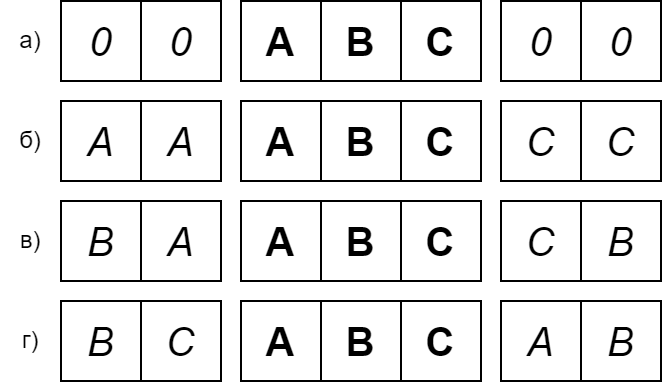
\includegraphics[scale=0.3]{images/paddings.png}
    \caption{Виды padding'ов: a) нулевой сдвиг, б) расширение границ, в) зеркальный сдвиг, г) циклический сдвиг}
\end{figure}

Заметим, что для трехмерной свертки требуется четырехмерное ядро, которое будет иметь размерность $D_{out}\times D_{in}\times K_W\times K_H$, так как изначально изображение имеет, например, $D_{in}=3$ канала для каждого цвета, но после применения свертки оно может иметь $D_out=16$ каналов.

\begin{figure}[htb]
    \centering
    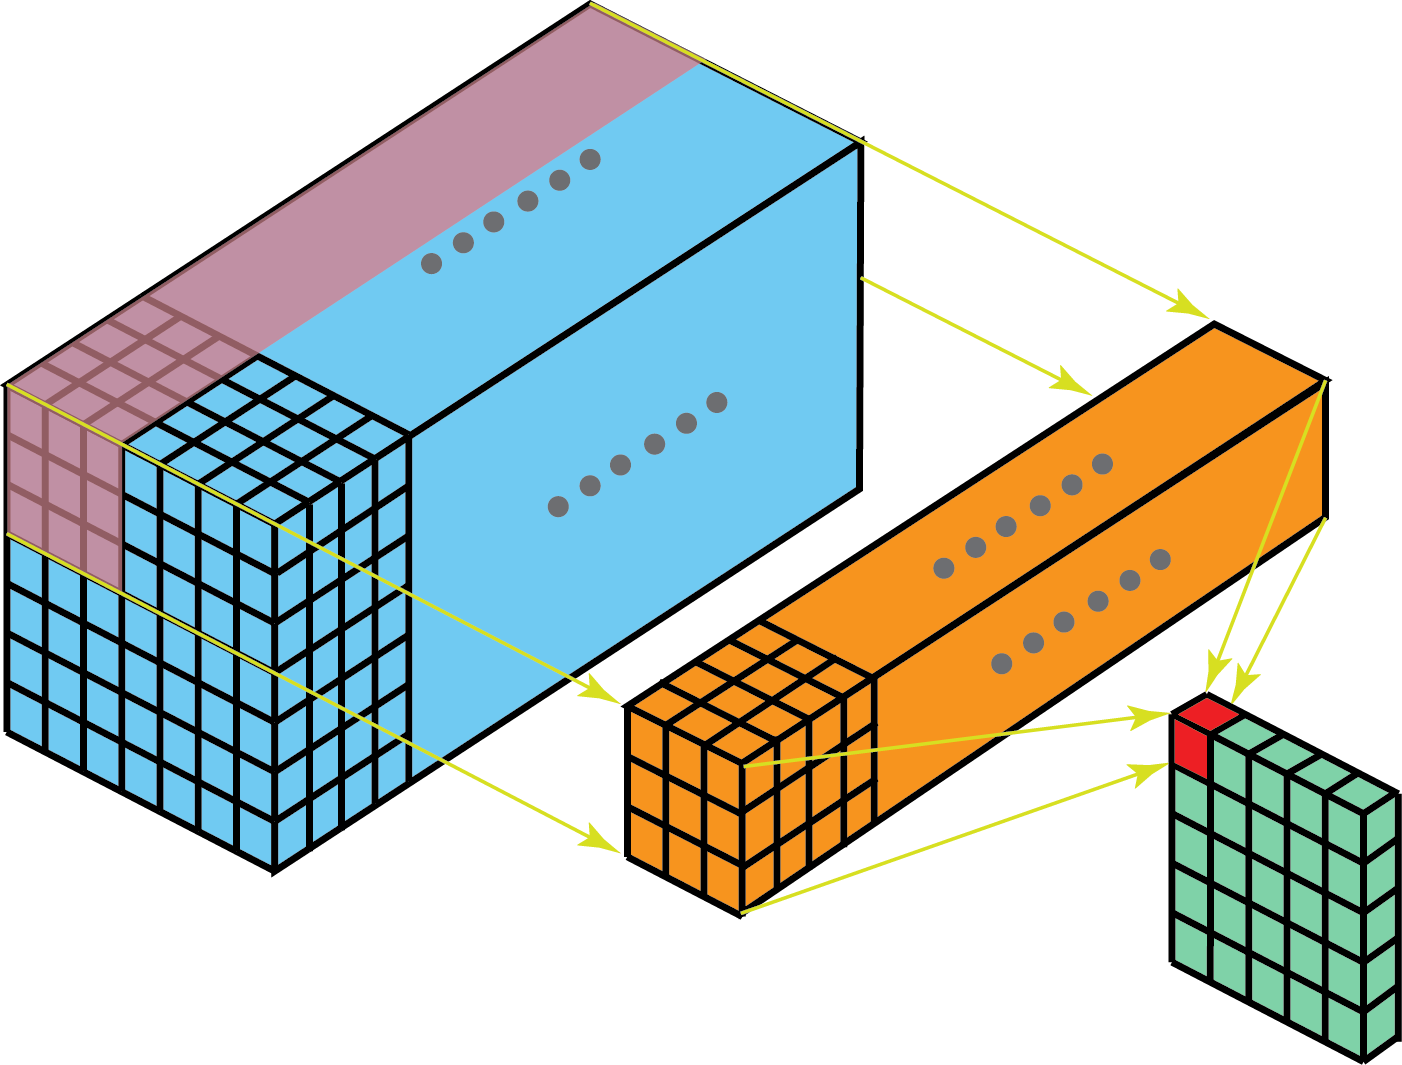
\includegraphics[scale=0.2]{images/3d-convolution.png}
    \caption{Пример 3D-свертки}
\end{figure}

\begin{remark}
    Размер после свертки пересчитывается по следующему правилу:
    \[
        O=\dfrac{I-K+2P}{S}+1,
    \]
    где
    \begin{itemize}
        \item $O$ -- размер выходного изображения
        \item $I$ -- размер входного изображения
        \item $K$ -- размер ядер, используемых в свёрточном слое
        \item $S$ -- сдвиг (stride)
        \item $P$ -- число элементов заполнения (padding)
    \end{itemize}
\end{remark}

\begin{definition}
    \textbf{Пулинг} (\textit{pooling}) --- свёрточное преобразование, которое используется для снижения размерности и декорреляции нейронов. Для пулинга используются обычно простые функции, такие как максимум или сумма, а шаг $S$ устанавливается достаточно большим (например, $S=K$). Формула для пересчета размера после пулинга:
    \[
        O=\dfrac{I-P_S}{S}+1,
    \]
    где
    \begin{itemize}
        \item $O$ -- размер выходного изображения
        \item $I$ -- размер входного изображения
        \item $S$ -- сдвиг (stride)
        \item $P_S$ -- число элементов пулинга в каждой итерации
    \end{itemize}
\end{definition}

\section{Обзор архитектур}

Примеры архитектур свёрточных сетей:
\begin{enumerate}
    \item Неокогнитрон Фукусимы (1980)
    \item LeNet (1998):
    \begin{itemize}
        \item Идеи иерархической структуры с соседних областей в сочетании с обратным распространением
        \item Небольшое число слоев
        \item Хорошо работает на MNIST
    \end{itemize}
    \item AlexNet (2014):
    \begin{itemize}
        \item Большая версия LeNet
        \item Размер свертки уменьшается (с $11\times11$ до $3\times3$) между входом и выходом
        \item Победа ImageNet2014 (по факту прорывом стала не архитектура, а то, что обучение сети впервые выполнялось на видеокарте)
    \end{itemize}
    \item VGG-16 и VGG-19 (2014):
    \begin{itemize}
        \item Большая версия AlexNet
        \item Вместо использования больших свёрток используются комбинации меньших сверток (вместо $5\times5$ дважды применяется $3\times3$)
        \item 138 и 144 млн. параметров соответственно
    \end{itemize}
    \item Сеть в сети (2014):
    \begin{itemize}
        \item Использует что-то более сложное, чем просто свёрточный слой
        \item Осталась теоретической
    \end{itemize}
    \item $1\times1$ свёртка (\textit{Cascaded Cross-Channel pooling}, \textit{CCCP}, \textit{каскадное кросс-канальное объединение}) позволяет играть с размерностью.
    \item Inception (2014):
    \begin{itemize}
        \item Идея: коррелированные нейроны будут сосредоточены в небольших областях. Чтобы определить это, мы можем использовать свёртку $1\times1$.
        \item Также попробуем искать их в областях $3\times3$ и $5\times5$.
        \item Вышеперечисленные фильтры можно объединять отдельным слоем.
    \end{itemize}
    \item ResNet (2015)
\end{enumerate}

\begin{figure}[htb]
    \centering
    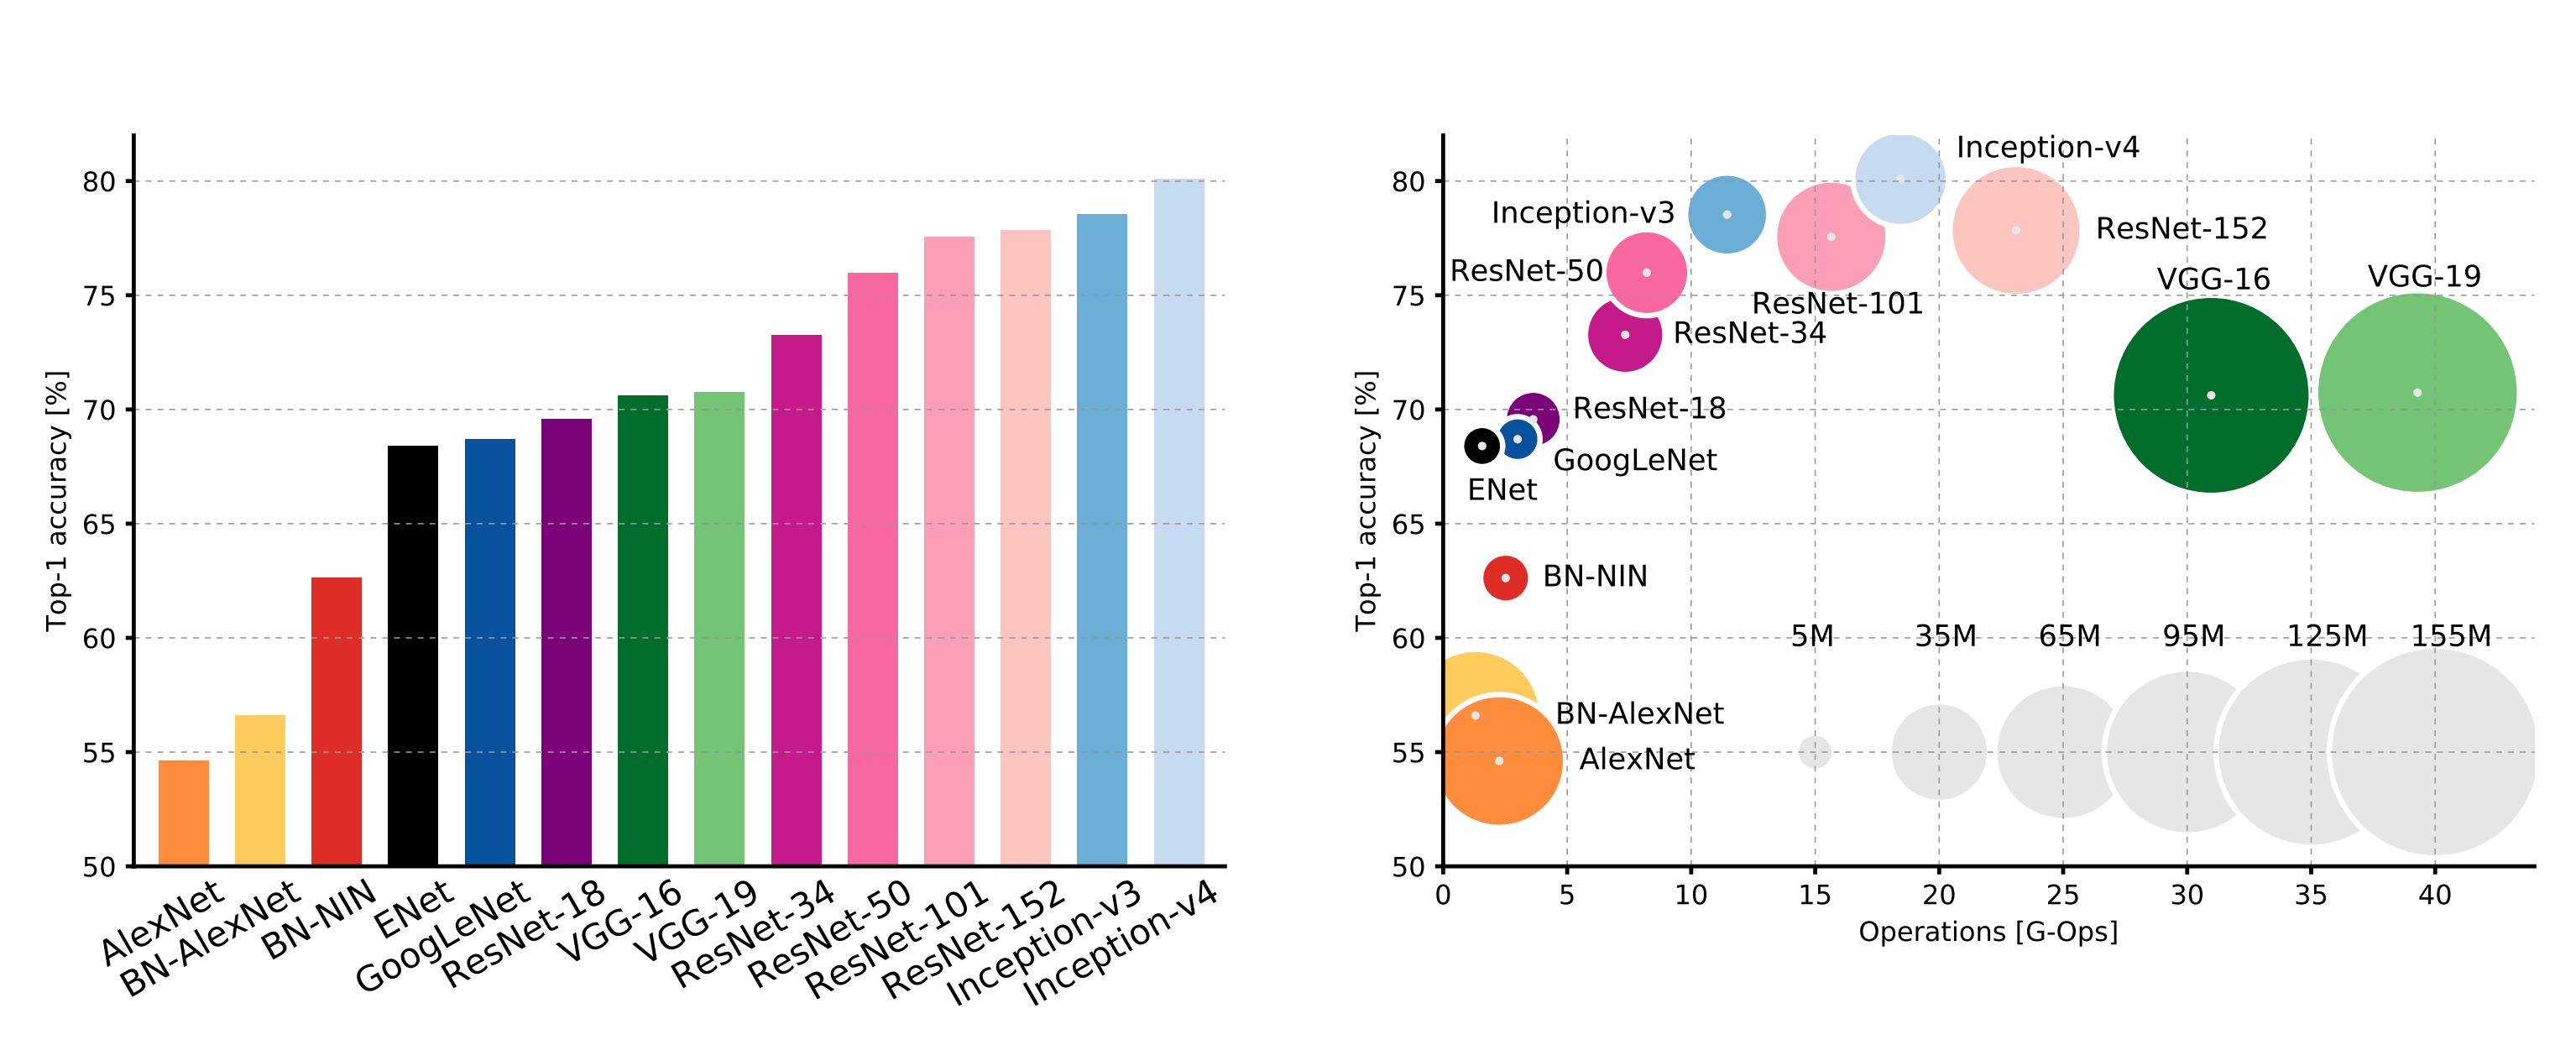
\includegraphics[scale=0.38]{images/cnn-comparison.png}
    \caption{Сравнение архитектур свёрточных сетей}
\end{figure}

\section{Задачи компьютерного зрения}

С помощью свёрточных сетей можно решать \textit{задачи классификации}:
\begin{itemize}
    \item MNIST -- первый набор данных для классификации. Содержит 10 классов, размер изображений -- $28\times28$, все изображения черно-белые и на них содержатся рукописные цифры.
    \item Fashion-MNIST -- современная замена MNIST с теми же характеристиками.
    \item CIFAR-10 -- содержит 10 классов, изображения цветные.
    \item Imagenet -- датасет с 1000 классов и минимум по 1000 изображений на каждый класс.
\end{itemize}

Второй класс задач -- это сегметнтация, детекция и так далее:
\begin{enumerate}
    \item Semantic segmentation
    \item Classification + Localization
    \item Object Detection
    \item Instance segmentation
\end{enumerate}

\begin{figure}[htb]
    \centering
    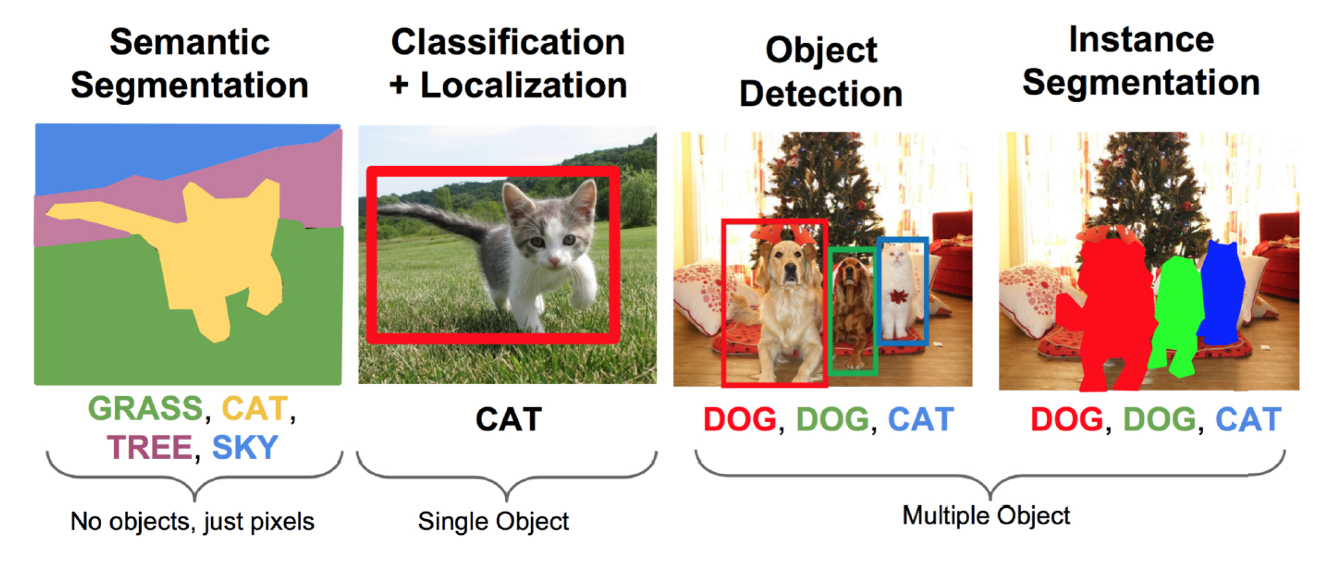
\includegraphics[scale=0.4]{images/up-conv-problems.png}
\end{figure}

\begin{remark}
    Такой класс задач решается сетями другими сетями (архитектурами), которые могут выполнять \textbf{деконволюцию} (увеличение изображения).
\end{remark}

\begin{figure}[htb]
    \centering
    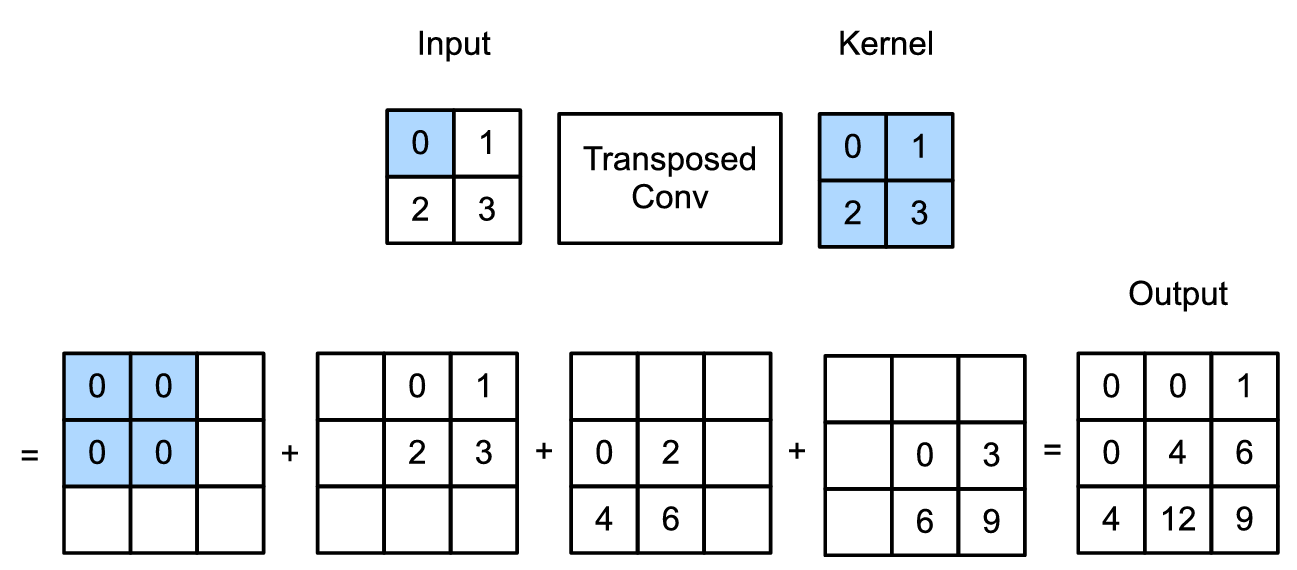
\includegraphics[scale=0.4]{./images/transposed-convolution.png}
    \caption{Transposed Convolution}
\end{figure}

Примеры современных решений для решения вышеперечисленных задач:
\begin{enumerate}
    \item Архитектура U-Net выполняет семантическую сегментацию
    \item Задачу распознавания решает R-CNN: архитектура, которая вырезает регионы изображения и прогоняет их через свёрточную сеть.
    \item YOLO - архитектура, похожая на обычную свёрточную архитектуру, но в результате получается тензор с числом классов и пятью дополнительными значениями для каждого региона: одно из них сигнализирует что что-то в регионе удалось найти, а остальные четыре задают координаты рамки.
\end{enumerate}